\documentclass[11pt,a4paper]{article}
\usepackage[T1]{fontenc}
\usepackage[utf8]{inputenc}
\usepackage{lmodern,microtype}
\usepackage{amsmath,amssymb,amsthm,mathtools,bm}
\usepackage{booktabs,array,tabularx,longtable}
\usepackage{graphicx,float,caption,xcolor}
\usepackage[margin=2.1cm]{geometry}
\usepackage{enumitem,fancyhdr}
\usepackage[hidelinks,pdfencoding=auto]{hyperref}

\hypersetup{
 pdftitle={FIN ST293--ST307: Active Feedback, Global Localization, and Observer Calibration},
 pdfauthor={Krzysztof Żuchowski},
 pdfsubject={Local mathematical continuation after FIN Release 10.76},
 pdfkeywords={FIN, active feedback, relative information, spontaneous localization, Stieltjes memory, D12 equivariants, trace class, calibration torsor, observer, validation}
}
\definecolor{proved}{RGB}{20,92,48}\definecolor{conditional}{RGB}{148,88,0}\definecolor{blocked}{RGB}{150,28,28}
\newcommand{\Proven}{\textcolor{proved}{\textbf{[PROVEN]}}}
\newcommand{\Evidence}{\textcolor{conditional}{\textbf{[STRONG NUMERICAL EVIDENCE]}}}
\newcommand{\Partial}{\textcolor{conditional}{\textbf{[PARTIAL]}}}
\newcommand{\Blocked}{\textcolor{blocked}{\textbf{[BLOCKED]}}}
\newtheorem{theorem}{Theorem}[section]
\pagestyle{fancy}\fancyhf{}\lhead{FIN ST293--ST307}\rhead{Release 10.77}\cfoot{\thepage}
\setlength{\headheight}{14pt}\setlist[itemize]{leftmargin=1.3em,itemsep=2pt,topsep=3pt}\sloppy

\begin{document}
\hypersetup{pageanchor=false}
\begin{titlepage}\centering
\vspace*{1cm}{\Large Fractal Information Theory Project\par}\vspace{.9cm}
{\huge\bfseries FIN ST293--ST307\par}\vspace{.35cm}
{\LARGE Active Feedback, Global Localization,\par}{\LARGE and Observer Calibration\par}
\vspace{1cm}{\large Analytical, interval, and bounded computational research report\par}
\vfill{\Large Krzysztof \.{Z}uchowski\par}\vspace{.2cm}
{\large Independent Researcher --- Fractal Information Theory Project\par}
{\large ORCID: 0009-0002-0909-3613\par}\vspace{.8cm}
{\large August 14, 2026\par}\vspace{.3cm}{\large Release 10.77\par}\vfill
\begin{minipage}{.92\textwidth}\small
\textbf{Repository snapshot.} The audited tracked base is commit
\texttt{bb540a767e210a5a3bf816e4868e7bcefbac3872}. The working tree contains
uncommitted research artifacts; the release manifest is required for reproducibility.

\medskip\textbf{License.} CC BY 4.0. \quad \textbf{Language.} English. \quad
\textbf{Resource type.} Preprint and executable reproducibility package.
\end{minipage}\end{titlepage}
\hypersetup{pageanchor=true}\pagenumbering{roman}

\begin{abstract}
Programs ST293--ST307 investigate the signed feedback left open by Release 10.76, the global
state landscape after that feedback is supplied, and the meaning of physical scale for an
observer inside a refinement layer.

The main theorem is a source obstruction. Every passive self-adjoint response
$C=f(A)\succeq0$ generates nonpositive modal growth in $\dot q=-Cq$. The positive
Stieltjes memory already constructed in FIN is another positive function of $A$ and only
increases stiffness. Therefore neither passive functional calculus nor passive memory can
generate the active term $-(g/2)\langle q,Aq\rangle$ required by the proposed information
instability. A pump, negative residue, nonequilibrium boundary condition, or another signed
state-dependent law remains necessary.

ST294 corrects the earlier lowest-mode intuition. On the full probability simplex, the
uniform-state Hessian first loses positivity at $g=12/\lambda_{\max}\approx5.12343$, not at
$12/\lambda_1\approx15.91256$. Moreover a pure vertex already has lower energy than the
uniform state for $g>2\log(12)/s\approx2.99331$. Thus global boundary localization can
precede every uniform Hessian instability. At supplied $g=4$, stratified multistart descent
finds strongly localized basins with all twelve peak labels and a positive numerical logit
Hessian; this is numerical evidence, not an existence or exhaustion theorem.

Further results include 160 consecutive outward-certified roots through the earlier
near-rank event, the analytic completion of the rank-two $D_{12}$ equivariant module, an
exact odd-dimensional Clifford obstruction, a three-output recovery SDP, a three-level
refinement cocycle retaining one free rate, a soft-infrared plateau tradeoff, and a theorem
that observer calibrations form a free positive torsor with no canonical absolute-scale
section. A complete 576-setting synthetic validation fixture passes syntax and is rejected
by the empirical gate. No independent raw events exist; ST307 remains blocked.

No strict source for active gain, selector closure, dimensional unit, Planck scale,
spacetime, legacy-role transfer, laboratory evidence, Standard Model, gravity,
$L_{\rm total}$, or Theory-of-Everything closure is claimed.
\end{abstract}
\tableofcontents\newpage\pagenumbering{arabic}

\section{Scope and proof discipline}

The strict operator remains
\[
A=sI-W,\qquad W_{xx}=0,\qquad W_{xy}=K_{\rm strict}(d(x,y))\quad(x\ne y),
\]
with $A\mathbf1=0$ and $A\succeq0$. The historical legacy kernel remains an intermediate
bridge object; no physical role is transferred from it. The ontology remains
informational nadsoliton $\to$ light $\to$ matter $\to$ emergent observer, with no lower
informational substrate. This ordering is not used as a proof premise.

\Proven{} denotes an exact theorem or outward finite certificate. \Evidence{} denotes a
reproducible numerical result without a global certificate. \Partial{} marks a finite subset
of an infinite or continuous problem. \Blocked{} records absent evidence.

\section{Executive ledger}
\small
\begin{longtable}{p{.075\textwidth}p{.22\textwidth}p{.60\textwidth}}
\toprule Program&Status&Result\\\midrule\endhead
ST293&\Proven&Passive $f(A)\succeq0$ and positive Stieltjes memory cannot source active negative-information gain.\\
ST294&\Proven{} + \Evidence&Exact threshold ordering; global simplex localization precedes the lowest-mode bifurcation.\\
ST295&\Evidence&At supplied $g=4$, all twelve peak labels have strongly localized numerical basins and one positive numerical Hessian.\\
ST296&\Proven&Positive memory loading commutes with $A$ and raises every positive modal stiffness.\\
ST297&\Proven&The free rank-two $D_{12}$ module persists for local real-analytic germs.\\
ST298&\Proven{} + \Partial&160 unique Krawczyk root boxes traverse the near event; a continuous tube is still absent.\\
ST299&\Proven&Three-output recovery reduces to a finite discrimination SDP, not one binary trace norm.\\
ST300&\Partial&Bounded likelihood ratios alone do not give a vanishing all-depth derivative tail.\\
ST301&\Proven{} + \Partial&Halfwidth $0.00075$ is the largest complete radius in the frozen campaign, not a global maximum.\\
ST302&\Proven&Exact anticommuting Hermitian involutions cannot exist in odd complex dimension.\\
ST303&\Proven{} + \Partial&Three-level exchange naturality leaves one common scale-rate modulus.\\
ST304&\Evidence&Finite-grid optimization of soft infrared plateau/trace tradeoffs.\\
ST305&\Proven&Observer calibrations form a free $(\mathbb R_+)^3$ torsor; invariant data select no absolute section.\\
ST306&\Proven&Complete synthetic conformance fixture passes syntax and permanently fails the empirical gate.\\
ST307&\Blocked&No independently registered child-resolved event record exists.\\
\bottomrule\end{longtable}\normalsize

\section{ST293 and ST296: the active-sign obstruction}

Release 10.76 studied
\[
V_g(p)=D(p\|u)-\frac g2\langle p-u,A(p-u)\rangle.
\]
The open issue was whether $g>0$ might emerge from existing FIN dynamics.

\begin{theorem}[passive functional-calculus no-go]
Let $C=f(A)$ be self-adjoint with $f(\lambda)\ge0$ on the spectrum of $A$. Then the
linear response $\dot q=-Cq$ has modal growth rates $-f(\lambda_k)\le0$. It cannot generate
an active negative quadratic stiffness.
\end{theorem}

The same applies to the certified-sign Stieltjes memory
\[
M=\sigma(0)I-\sum_jr_j(A+c_jI)^{-1},\qquad c_j,r_j>0.
\]
It commutes with $A$, is positive semidefinite, and $A+\epsilon M$ raises the minimum
positive stiffness from $0.754121$ at $\epsilon=0$ to $0.962014$ at $\epsilon=2$. Passive
memory therefore moves the system away from, not toward, the desired instability.

This is a class theorem, not a universal impossibility theorem. Active, nonnormal,
state-dependent, negative-residue, pumped, or nonequilibrium laws remain possible. But any
such law must expose its source and sign; calling it ``information feedback'' is not enough.

\section{ST294--ST295: the global simplex overturns the lowest-mode picture}

At the uniform state, the tangent Hessian is
\[
H_u(g)=12I-gA.
\]
Consequently mode $k$ loses local stability at $g_k=12/\lambda_k$. The first loss is at
\[
g_{\rm Hess}=\frac{12}{\lambda_{\max}}=5.123427551398615,
\]
while the lowest positive carrier destabilizes only at
\[
g_1=\frac{12}{\lambda_1}=15.912562501468873.
\]
There is an even earlier energetic comparison. For a pure vertex $e_j$,
\[
V_g(e_j)=\log12-\frac{g}{2}s,
\]
so vertices beat the uniform value zero when
\[
g>g_E=\frac{2\log12}{s}=2.9933093488992286.
\]
Hence
\[
g_E<g_{\rm Hess}<g_1.
\]

\begin{figure}[H]\centering
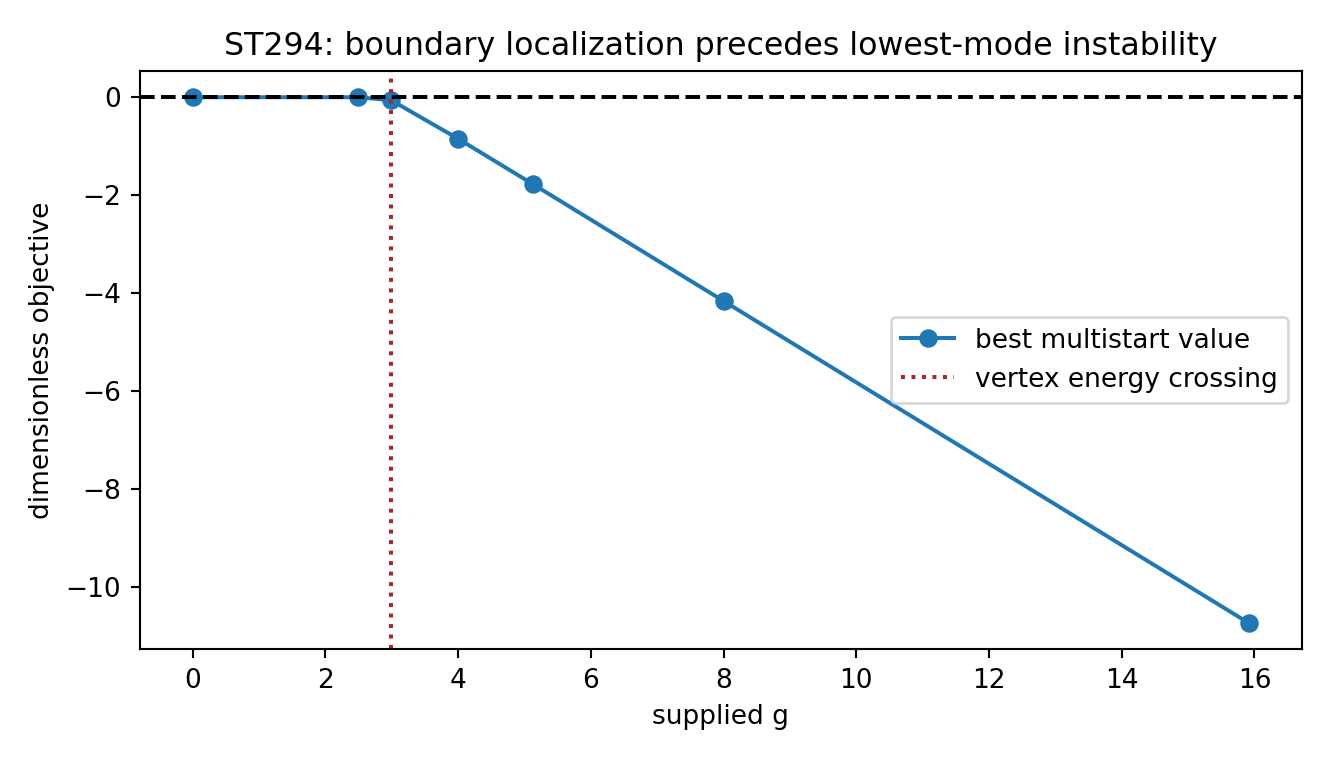
\includegraphics[width=.78\textwidth]{FIN_ST293_ST307_Figures/st294_global_competition.png}
\caption{The global objective becomes localization-favouring before the lowest-mode carrier destabilizes.}
\end{figure}

This refutes the interpretation that the degree-twelve lowest-carrier term is the first
global state selector. It remains the first angular anisotropy on that restricted carrier,
but boundary states compete earlier on the full simplex.

At supplied $g=4$, 192 peak-stratified numerical descents reach strongly localized endpoints
and represent all twelve peak labels. A representative maximum probability is about $0.9902$,
and its finite-difference logit Hessian has strictly positive sampled eigenvalues. This is
strong evidence for localized basins but not a theorem of exactly twelve stationary minima,
global optimality, orbital stability, or physical vacuum selection.

\section{ST297--ST300: response completion, continuation, and recovery boundaries}

ST297 extends the polynomial classification. Every local real-analytic equivariant germ is
uniquely of the form
\[
F(z)=a(|z|^2,\Re z^{12})z+b(|z|^2,\Re z^{12})\bar z^{11},
\]
where $a,b$ are real-analytic germs. Singular, merely smooth, nonlocal, and history-dependent
maps remain outside this theorem.

ST298 inserts 160 consecutive pseudo-arclength sections around the earlier near-rank event.
Every root is unique in an outward Krawczyk box. The smallest point singular value is
$2.9624\times10^{-6}$ at fine step 85 and then reopens.

\begin{figure}[H]\centering
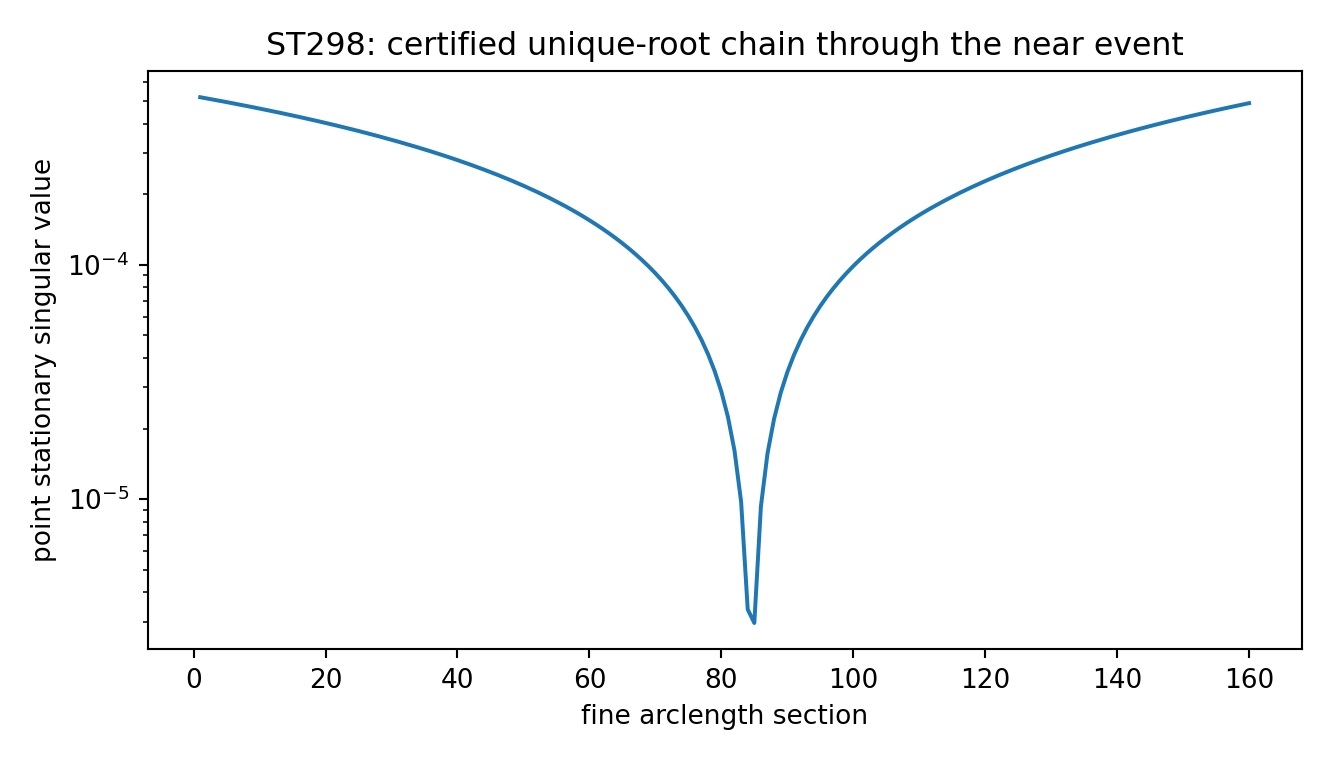
\includegraphics[width=.75\textwidth]{FIN_ST293_ST307_Figures/st298_near_event.png}
\caption{A certified chain of unique roots resolves the sampled near event; it is not yet a continuous tube.}
\end{figure}

ST299 shows that recovery from three measure-and-prepare outputs is exactly the state-
discrimination semidefinite program
\[
\max\sum_i\operatorname{tr}(M_i\tau_i),\quad M_i\succeq0,\quad\sum_iM_i=I,
\]
with dual $\min\operatorname{tr}\Gamma$ subject to $\Gamma\succeq\tau_i$. For noncommuting
triples, no single signed difference operator supplies all effects; the binary trace-norm
formula does not extend unchanged.

ST300 finds that bounded one-step likelihood ratios yield derivative bounds growing with
unresolved depth. Without a uniform projective contraction or spectral-gap estimate, they do
not produce a vanishing derivative tail. The finite-depth Chernoff bracket therefore remains
finite-depth.

\section{ST301--ST304: bounded certification and multiscale refinement}

Under the frozen 500,000-call ledger, halfwidth $0.00075$ is the largest fully completed
nuisance cube. Corner screens at $0.00080$, $0.00090$, and $0.00100$ fail at the old base
resolution. They do not show root loss and are not complete covers; the result is campaign-
relative, not a maximal-radius theorem.

Two exact Clifford facts now align: ST286 gives even-dimensional counterexample lifts, while
ST302 proves odd-dimensional impossibility. If invertible involutions satisfy $XZ=-ZX$ in
dimension $d$, determinants imply
\[
\det(XZ)=(-1)^d\det(XZ),
\]
which is impossible for odd $d$.

At three binary refinement levels the complement is a Kronecker sum with rates
$v_1,v_2,v_3$. Coassociativity alone leaves all three. Naturality under the full $S_3$
exchange of indistinguishable levels forces $v_1=v_2=v_3=v$, but does not choose $v$.
Thus a consistent constant scale cocycle appears, not an absolute physical scale.

ST304 explores soft infrared profiles
\[
q_{\alpha,a}(\mu)=\left(\frac{\mu}{\mu+a}\right)^\alpha.
\]
Under heat-trace budget $5$ and a $2\%$ plateau tolerance, the best frozen grid point is
$\alpha=2$, $a=2^{-10}$, heat trace $4.6852$, and logarithmic plateau width $9.4479$.

\begin{figure}[H]\centering
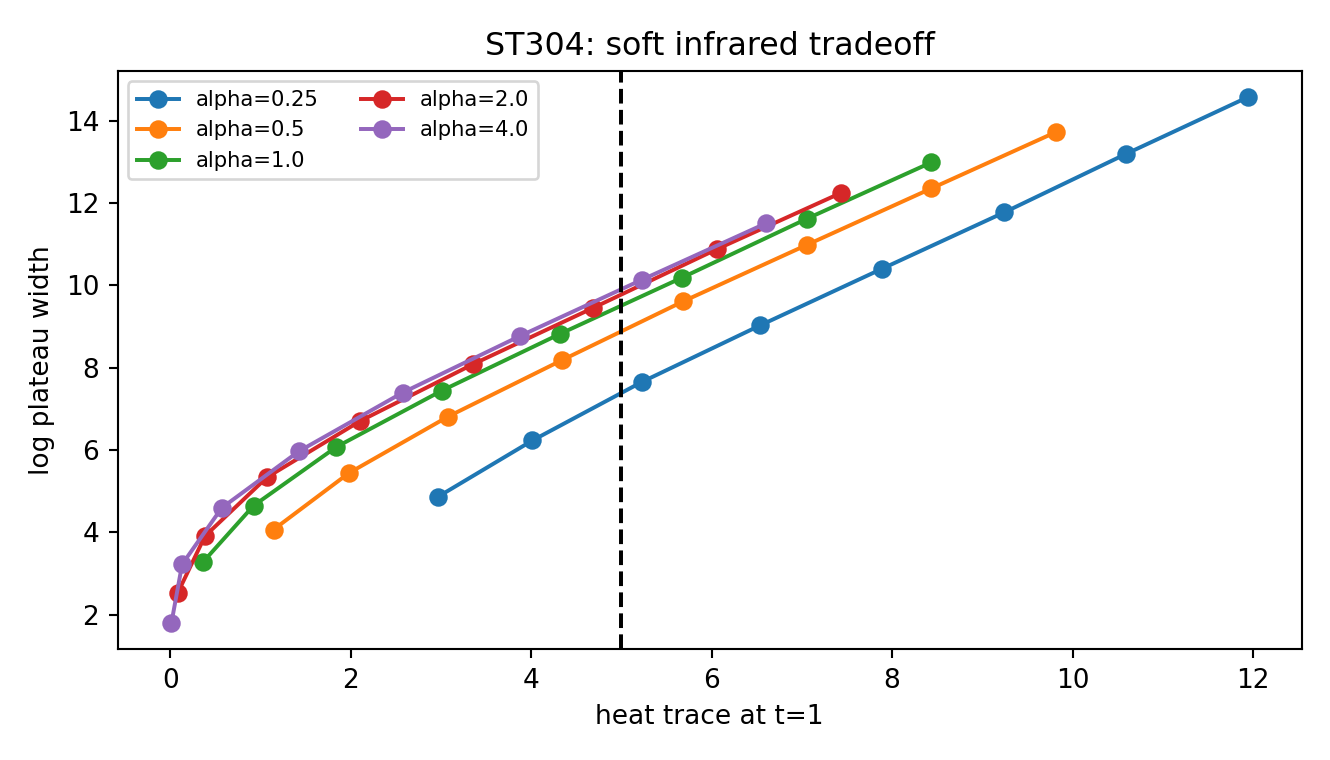
\includegraphics[width=.78\textwidth]{FIN_ST293_ST307_Figures/st304_soft_ir_tradeoff.png}
\caption{Soft infrared profiles trade heat trace for a finite near-Haar visibility window.}
\end{figure}

This is a family/grid result, not a continuum extremizer theorem or a derivation of the
profile from FIN.

\section{ST305: observer-relative units as a calibration torsor}

For each layer $n$, let an operational observer context be
\[
\mathfrak O_n=(\mathcal H_n,A_n,\mathcal P_n,\mathcal M_n,\omega_n,
\mathcal C_n,\mathcal R_n).
\]
Calibration choices $(\ell_n,\tau_n,\varepsilon_n)$ form a principal
$G=(\mathbb R_+)^3$ torsor. Under $G$, dimensionless length, time, and energy ratios have
weight zero, while absolute quantities have nonzero weights. Transition maps satisfy the
cocycle law
\[
g_{kn}=g_{km}g_{mn}.
\]

\begin{theorem}[no canonical absolute calibration from invariant data]
If the calibration torsor is free, dimensionless $G$-invariant FIN data cannot select a
distinguished point of it. A dimensional anchor for each independent unit direction, or
relations reducing $G$, is necessary.
\end{theorem}

This makes the user's internal-observer intuition mathematically precise. An observer can
construct invariant local ratios and compare layers through a cocycle. Living inside a
layer does not generate metres, seconds, or joules. It makes the absence of absolute scale
operationally unobservable until a comparison or calibration is supplied.

\section{ST306--ST307: conformance is not experiment}

ST306 creates all $24\times24=576$ child-resolved setting rows. The frozen validator accepts
the schema and complete coverage. When the empirical flag is requested, it rejects the file
because it is marked synthetic. The permanent status is
\texttt{PERMANENT\_NON\_EVIDENCE}.

No independently registered ST307 raw-event record exists. Empirical analysis remains
\Blocked. This is an evidentiary boundary, not a negative experiment.

\section{Falsification ledger and deepest surviving interpretation}
\begin{longtable}{p{.28\textwidth}p{.31\textwidth}p{.34\textwidth}}
\toprule Claim&Falsification test&Surviving statement\\\midrule\endhead
Passive memory may create active gain&Spectral sign audit&False for positive Stieltjes memory; it raises stiffness.\\
The lowest mode is the first global selector&Full-simplex Hessian and vertex comparison&False; boundary localization can win first.\\
Exactly twelve basins are proved&Stratified numerical search&All labels appear, but existence and exhaustion remain numerical.\\
The polynomial module misses analytic responses&Convergent series grouping&The same rank-two module persists for analytic germs.\\
The near event is a fold&160 outward root boxes&No sampled fold; a continuous tube is still missing.\\
Binary recovery formula generalizes directly&Three noncommuting outputs&The correct object is an SDP.\\
Three-level refinement selects scale&Full level exchange&One common modulus survives.\\
An internal observer generates absolute units&Calibration-group action&Only ratios are invariant; no canonical section exists.\\
Complete synthetic data are evidence&Empirical validator mode&False; permanent rejection is intentional.\\
\bottomrule\end{longtable}

The deepest interpretation surviving this batch is:
\begin{quote}
FIN's strict self-adjoint operator and passive memory organize stable relational dynamics but
do not generate the active sign needed to destabilize information equilibrium. If that sign
is added, the full state space localizes at its boundary before the lowest spectral phase
circle becomes the first instability. Across refinement layers, an internal observer has
well-defined dimensionless relations and cocycle-consistent comparisons, but absolute units
remain a choice in a free calibration torsor. The missing physical bridge is therefore not
one scalar: it is an active nonequilibrium source together with operational calibration and
an independent record.
\end{quote}

\section{Recommended programs ST308--ST322}
\begin{enumerate}
\item[\textbf{ST308}.] Classify the smallest active state-dependent laws compatible with
$D_{12}$ covariance, positivity of probabilities, and a transparent energy budget.
\item[\textbf{ST309}.] Test whether a finite pumped auxiliary variable can generate $g>0$
after elimination without importing a broken phase.
\item[\textbf{ST310}.] Derive a passivity/active-gain dichotomy for general nonnormal memory
realizations and identify the minimum nonequilibrium resource.
\item[\textbf{ST311}.] Obtain interval existence certificates for one localized $g=4$
simplex stationary point and generate its twelve translation images exactly.
\item[\textbf{ST312}.] Prove or refute global minimality of the localized orbit over the full
simplex using convex envelopes or branch-and-bound.
\item[\textbf{ST313}.] Continue the localized family in $g$ and locate the first-order
energy crossing relative to the uniform state.
\item[\textbf{ST314}.] Construct a continuous validated tube across the ST298 fine chain or
produce an explicit section gap.
\item[\textbf{ST315}.] Solve one rational three-output recovery SDP exactly and identify its
minimal algebraic field.
\item[\textbf{ST316}.] Seek a uniform Hilbert/projective contraction certificate for the
Chernoff transfer operator; stop if a counterexample occurs.
\item[\textbf{ST317}.] Allocate the fixed nuisance-cover budget adaptively using certified
margin predictors, without interpreting failure as root loss.
\item[\textbf{ST318}.] Classify approximate odd-dimensional Clifford pairs and prove a
dimension-dependent anticommutator lower bound.
\item[\textbf{ST319}.] Test whether a nonconstant three-level scale cocycle is compatible
with full refinement coherence or is gauge-equivalent to the constant modulus.
\item[\textbf{ST320}.] Prove an extremal theorem for soft infrared profiles under a heat-
trace budget, beyond the ST304 finite grid.
\item[\textbf{ST321}.] Reduce the calibration structure group using declared cross-channel
relations and count the remaining independent dimensional anchors.
\item[\textbf{ST322}.] Resume empirical analysis only after independently registered,
hashed, child-resolved raw events exist.
\end{enumerate}

ST308--ST310 have highest priority: the active sign must be derived with its resource ledger
or retained as an axiom. ST311--ST313 then determine whether the numerically localized orbit
is a genuine theorem-level phase. ST321 is the most direct continuation of the internal-
observer idea: it asks how many calibrations remain after all legitimate channel relations,
not whether observation alone manufactures a unit.

\section{Reproducibility and conclusion}

The source \texttt{fin\_st293\_st307\_research.py} writes fifteen packets, an aggregate JSON,
a CSV ledger, a complete synthetic conformance fixture, and three figures. The independent
suite \texttt{test\_fin\_st293\_st307.py} performs sixteen live checks of hashes, spectral
signs, threshold identities, basin-label coverage, memory monotonicity, all 160 Krawczyk
boxes, the noncommuting recovery example, bounded tail stop, campaign boundary, determinant
obstruction, refinement permutation law, soft-profile feasibility, calibration weights,
synthetic empirical rejection, and the ST307 stop. All sixteen tests pass.

The current state is sharper than Release 10.76. Relative information explains the first
allowed angular anisotropy, but current passive FIN dynamics cannot supply the active sign
that makes it operative. Once a coupling is supplied, global state competition favours
strong localization rather than making the lowest phase carrier automatically fundamental.
The observer-layer hypothesis survives in a precise relational form, while its strongest
version---internal production of absolute units---is obstructed by the calibration torsor.

\end{document}
